\documentclass[12pt]{article}
\usepackage{graphicx}

\begin{document}
\title{Remarks on VLR}
\author{AAD}
\date{May 10, 2020}
\maketitle

\section{Introduction}

Variable load risk (VLR) is one part in the financial management of
a load serving contract.  For one temporal period (usually taken to be
one hour), unit VLR in \$/MWh is defined as 
 
\begin{equation}
  VLR = (T - P)(\frac{L}{L_{wn}} - 1)
\end{equation}

where $T$ is the tariff price, $P$ is the energy price of this period,
$L$ is the load in this period, and $L_{wn}$ is the weather normal
load.  As a convention, load values are taken to be positive. 

Given that both $P$ and $L$ are random variables, the mean $VLR$ can
be shown to be
\begin{equation}
  E[VLR] = -\frac{\mathrm{Cov}(L,P)}{E[L]} = -\frac{\sigma_P \sigma_L}{E[L]} \rho
\end{equation}
where $\sigma_P$, $\sigma_L$ is the standard deviation of the price
and load respectively, $\rho$ is the correlation between load and
price.

VLR mean does not depend on the tariff price $T$ and will equal zero
if the correlation between load and price is zero.  Also, as price
volatility increases, VLR mean also increases.

Note that a low VLR mean does not imply a small financial risk.  So
how to price a random variable with a small mean but large variance?
Is the concept of VLR delta $\Delta = d\mathrm{VLR}/dP$ useful in managing VLR
risk?  Below, we discuss cases that shed more insight into these
questions.

\section{Deterministic relationship between price and load}

In general, the joint distribution of price and load cannot be
expressed in closed analytical form.  To gain more insight we consider
in this section the case when price is a deterministic function of
load only.  We discuss relaxing this constraint in the next section.

Let's denote the relationship between load and price by the function
$P=S(L)$.  We can think of function $S(L)$ as representating the
generation stack.

VLR as a function of market price $P$ is a concave function with two
zeros.  One zero is trivial and happens when market price equals the
tariff price $T$.  To find the other zero we recognize that the stack
function $S$ is invertible, so there will be a price for which
$S^{-1}(P) = L_{wn}$.  This price will be the second zero of the VLR
function.  In general, this second zero is close to the market price
$P$.

It is reasonable to expect that for various load ranges, there is a
linear relationship btween price and load.  For simplicity, take the
load to be a normally distributed random variable.  First, consider
the linear model
\begin{eqnarray}
  L &=& {\cal N}(L_{wn}, \epsilon_L)  \\
  P &=& a L + b,
\end{eqnarray}

and an adjusted linear model with quadratic tail.  For moderate loads,
there is a linear relationship between load and price, but for higher
loads, this linear relationship becomes quadratic.  This quadratic
tail model is more realistic for dynamic of power prices.
\begin{eqnarray}
  L &=& {\cal N}(L_{wn}, \epsilon_L)  \\
  P &=& a L + b + c(L-L_*)^2\mathrm{max(L-L_*,0)}.
\end{eqnarray}

Let's look at a concrete example.  With tariff $T=70$ \$/MWh, $L_{wn}
= 600$ MWh.  Take $\epsilon_L = 30$ MWh, which corresponds to $0.05\%$
of the $L_{wn}$ value.  Using $a=0.04$ and $b=4$, the price
distribution of the linear model is ${\cal N}(28,1.2^2)$.  The
quadratic tail model is $P = 0.04L + 4 +
0.02*\mathrm{max}(L-L_*,0)(L-L_*)^2$ with $L_*=650$.  Prices grow
linearly as a function of load up to $95\%$ probability level, after
which they grow quadratically for top $5\%$ probability.

For the linear model, $\mathrm{VLR}(P)$ is a quadratic.  It has zeros at the
tariff price $T$ and at $E[P]$.  The VLR delta is trivially computed
to be
\begin{equation}
  \Delta = \frac{d\mathrm{VLR}}{dP} = \frac{a}{2E[L]}(P_* - P) 
\end{equation}
where $P_*$ is the price for the vertex of the VLR function. 

\begin{figure}[htb]
\begin{center}
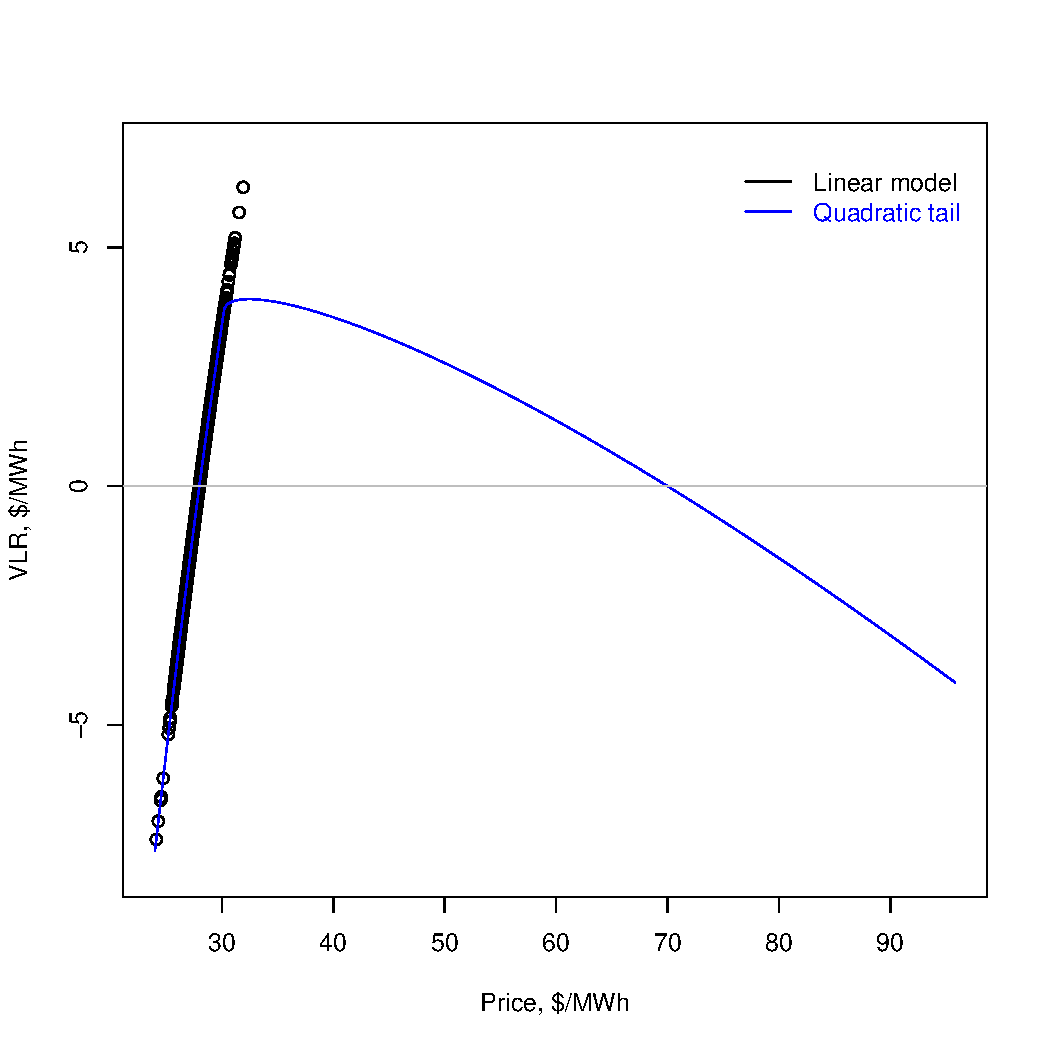
\includegraphics[height=4in,width=4in,angle=0]{img/vlr_vs_price.pdf}
\caption{VLR as a function of price when prices are a deterministic
  function of load.  Hard to see from the figure, but the linear model
  is a quadratic, with the second zero at the tarrif price of
  \$70/MWh. The prices for the linear model shown as points,
  correspond to 1000 values of load ${\cal N}(600,30)$ by the linear
  transformation $P=0.04*L + 4$.  The quadratic tail model (blue) has
  prices equal $P = 0.04L + 4 + 0.02*\mathrm{max}(L-L_*,0)(L-L_*)^2$
  with $L_*=665$. The vertex price for the linear model is $P_*=49$,
  half way between $E[P]$ and the tariff price $T$.  For the quadratic
  tail model, the VLR for the bottom $95\%$ of the prices are the same
  as of the linear model.}
\label{vlrVsPrice}
\end{center}
\end{figure}


This formula indicates that as prices are below the vertex price $P_*$ and
increasing, VLR delta decreases.  And as prices increase above the
vertex price $P_*$ delta becomes more and more negative.  This is
exactly a short Gamma $\Gamma$ position.  The $\Gamma = -a/E[L]$
is independent of price level.

\begin{table}[ht]
\centering
 \label{summaryVlr}
 \begin{tabular}{rrrrrrr}
  \hline
 & Min. & 1st Qu. & Median & Mean & 3rd Qu. & Max. \\ 
  \hline
  $VLR_0$ & -0.65 & -0.08 & -0.02 & -0.06 & -0.01 & -0.00 \\
  $VLR_1$ & -7.39 & -1.48 & -0.09 & -0.06 & 1.45 & 6.25 \\
  $VLR_2$ & -8.88 & -1.50 & - 0.10 & -0.12 & 1.37 & 3.62 \\
   \hline
 \end{tabular}
 \caption{Summary VLR distribution.  $VLR_0$ is calculated using
   $E[P]=28$ instead of the tariff price $T$, $VLR_1$ is calculated
   using the linear model and the actual tariff price $T=60$, $VLR_2$
   is calculated using the quadratic tail model.  As expected, the VLR
   mean for $VLR_0$ and $VLR_1$ are equal.  }
\end{table}


\section{Stochastic relationship between price and load}

In general, price formation depends on a variety of other variables
in addition to load, for example fuel prices, different unit
availability, import/exports from other regions, etc.

So a more realistic model builds on the quadratic tail model and adds
a multiplicative stochastic component to it.   

\begin{eqnarray}
  L &=& {\cal N}(L_{wn},\sigma_L^2)  \\
  P &=& (a L + b + c(L-L_*)^2\mathrm{max(L-L_*,0)})(1 + {\cal N}(0,\sigma_P^2)).
\end{eqnarray}




\end{document}
